\documentclass[tikz,border=4pt]{standalone}
\usepackage{amsmath}
\begin{document}
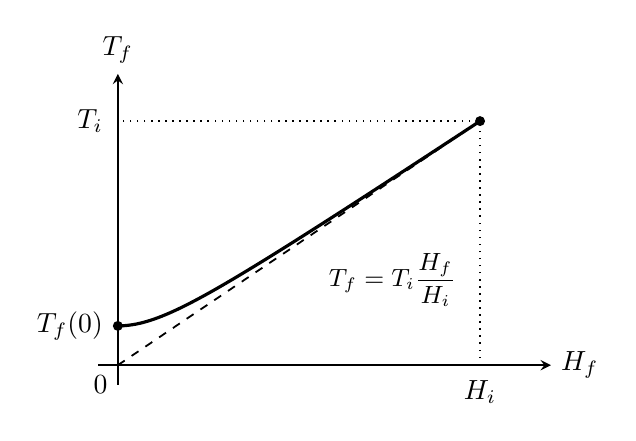
\begin{tikzpicture}[>=stealth, thick, scale=1.0]
  % Axes: H_f from 0 to 5.2, T_f from 0 to 3.6
  \draw[->, line width=0.65pt] (-0.25, 0) -- (5.5, 0) node[right] {$H_f$};
  \draw[->, line width=0.65pt] (0, -0.25) -- (0, 3.7) node[above] {$T_f$};
  \node[below left] at (0, 0) {$0$};

  % H_i = 4.6, T_i = 3.1, eps = 0.75 (represents |J| sqrt(z/2) / mu)
  % Curve: T_f(x) = 3.1 * sqrt((x^2 + 0.75^2)/(4.6^2 + 0.75^2))
  % At x=0: y = 3.1 * 0.75 / 4.6607 = 0.499
  \draw[dashed, line width=0.65pt] (0, 0) -- (4.6, 3.1);
  \draw[dotted, line width=0.55pt] (4.6, 0) -- (4.6, 3.1) -- (0, 3.1);

  \draw[line width=1.15pt, domain=0:4.6, samples=100, smooth]
    plot (\x, {3.1 * sqrt((\x*\x + 0.75*0.75)/(4.6*4.6 + 0.75*0.75))});

  % Endpoint dots
  \fill (0, 0.499) circle (1.8pt);
  \fill (4.6, 3.1) circle (1.8pt);

  % Axis labels
  \node[below] at (4.6, -0.06) {$H_i$};
  \node[left] at (-0.06, 3.1) {$T_i$};
  \node[left] at (-0.06, 0.50) {$T_f(0)$};

  % Dashed line annotation
  \node[font=\small, below right] at (2.55, 1.55) {$T_f = T_i \dfrac{H_f}{H_i}$};
\end{tikzpicture}
\end{document}
